% Computational companion to the numerical-reliability CSDA draft.
% Uses author-provided Elsevier CAS Bundle v2.4, copied verbatim by CI.
\documentclass[a4paper,fleqn]{cas-dc}
\usepackage[authoryear,longnamesfirst]{natbib}
\usepackage{amsmath,amssymb,amsthm,mathtools}
\usepackage{graphicx,booktabs,url}
\usepackage{hyperref}
\hypersetup{colorlinks=true,urlcolor=blue,citecolor=blue,linkcolor=blue}
\newcommand{\R}{\mathbb R}
\newcommand{\tr}{\operatorname{tr}}
\newcommand{\RSS}{\operatorname{RSS}}
\newcommand{\edf}{\operatorname{edf}}
\newcommand{\CV}{\operatorname{CV}}
\newcommand{\GCV}{\operatorname{GCV}}
\newcommand{\diag}{\operatorname{diag}}
\begin{document}
\let\WriteBookmarks\relax
\def\floatpagepagefraction{1}
\def\textpagefraction{.001}
\shorttitle{Computation with smoothness-indexed PLS}
\shortauthors{Espino-Montelongo and Cort\'es-Toto}
\title[mode=title]{Computational costs of smoothness-indexed penalized least squares: spectral reuse, cached grids and solver trade-offs}
% Provisional authorship and order; confirm together before submission.
\author[1]{Heriberto Espino-Montelongo}
\author[1]{Daniela Cort\'es-Toto}
\affiliation[1]{organization={Universidad de las Am\'ericas Puebla},
 city={San Andr\'es Cholula},state={Puebla},country={Mexico}}
\begin{abstract}
Finite-difference penalized least squares is most often tuned through a penalty $\lambda$ whose numerical scale varies with series length and difference order. We study the computational cost of using instead normalized trace smoothness $s\in[0,1]$ for any $1\le d<n$ and a fixed, possibly nonzero, mean of the penalized differences. A singular-value representation gives an invertible $s\leftrightarrow\lambda$ map and permits caching of spectra, data projections and grids across criteria and independent series. We distinguish single fitted curves, single criterion scores, repeated full-grid searches and multi-series reuse, and derive arithmetic and memory complexity for dense solves, dense Cholesky, general banded solves, banded Cholesky, dense eigendecomposition and SVD. We analyze an archived 80,640-row paired Windows benchmark with seven numerical backends, five criteria, eight search policies, two fixed means, two sample sizes and two seeds. In a representative $n=48,d=2$ five-criterion experiment, repeated native-smoothness mapping took 11.234 ms, against 3.980 ms when a mapped grid was shared, a descriptive 2.82-fold reduction. Native-$s$ and pretranslated searches select identically when they evaluate identical penalties; an independent logarithmic penalty grid is not the same statistical candidate set. Separate repeated-fit and 20-seed solver benchmarks show that the fastest method depends on workload and numerical-validity requirements. Timings measure the archived machine and are not universal complexity proofs. This computational companion will ultimately be combined with a separate high-precision study to characterize accuracy--runtime trade-offs.
\end{abstract}
\begin{keywords}
Smoothness index \sep penalized least squares \sep algorithmic complexity \sep caching \sep spectral decomposition \sep computational benchmarking \sep cross-validation
\end{keywords}
\maketitle
\section{Introduction and smoothness coordinate}\label{sec:foundation}
Quadratic finite-difference penalized least squares (PLS) has a long history in Whittaker--Henderson smoothing \citep{whittaker1923,guerrero2007}. The penalty $\lambda$ is mathematically convenient, but the same numerical value need not express the same smoothness for different difference orders or sample lengths. Guerrero's trace-based smoothing measure \citep{guerrero2008} and its use with CV, GCV, AICc and BIC \citep{cortes2017} are established precedents. We do not claim to invent the smoother or its tuning criteria; instead, we investigate the \emph{computational cost of an interpretable bounded coordinate and the reuse of its mapping across many evaluations}.

For $y\in\R^n$, difference order $1\le d<n$, and fixed mean of the penalized differences $\mu$, let $D_d\in\R^{(n-d)\times n}$ denote forward differences and define
\begin{equation}\label{eq:pls}
\widehat\tau_{\lambda,\mu}
=\arg\min_\tau\{\|y-\tau\|_2^2+
\lambda\|D_d\tau-\mu\mathbf1\|_2^2\}.
\end{equation}
Put $r=n-d$, $Q_d=D_d^\top D_d$, and $H_\lambda=(I+\lambda Q_d)^{-1}$. A polynomial particular solution is $p_{\mu,t}=\mu\binom{t-1}{d}$, and $\widehat\tau=p_\mu+H_\lambda(y-p_\mu)$. The penalty has a $d$-dimensional polynomial nullspace, so $\tr(H_\lambda)\to d$ as $\lambda\to\infty$.

Write $\delta_1,\ldots,\delta_r>0$ for the positive eigenvalues of $Q_d$. We use the normalized smoothness index
\begin{equation}\label{eq:S}
S_d(\lambda)=\frac{n-\tr(H_\lambda)}{n-d}
=\frac1r\sum_{j=1}^{r}\frac{\lambda\delta_j}{1+\lambda\delta_j}.
\end{equation}
Each $\delta_j>0$ implies $S_d'(\lambda)=r^{-1}\sum_j\delta_j/(1+\lambda\delta_j)^2>0$, hence $S_d$ is continuous, strictly increasing, and maps $[0,\infty]$ onto $[0,1]$. Every interior $s$ has a unique penalty $\Lambda_{n,d}(s)$. The map depends only on $(n,d)$, \emph{not} on observations or the fixed reference mean $\mu$. Therefore it can be cached across different series, criteria and $\mu$ values. The denominator $n-d$ normalizes an established trace-based index; it is not a new statistical model.

\subsection{Shift-free full spectral reconstruction}
Let $D_d=U\diag(\sigma)V^\top$ be a reduced SVD over the $r$ positive singular modes and write $w_j=\lambda\sigma_j^2/(1+\lambda\sigma_j^2)$. A numerically useful identity is
\begin{equation}\label{eq:shiftfree}
\begin{aligned}
\widehat\tau_{\lambda,\mu}
=y-V\bigl[&w\odot(V^\top y)\\
&-\mu(w\oslash\sigma)\odot(U^\top\mathbf1)\bigr],
\end{aligned}
\end{equation}
where multiplication and division are componentwise. It avoids forming the potentially enormous polynomial $p_\mu$ at high $d$ and costs $O(nr)$ for a complete curve once the SVD is available. A separate high-precision companion manuscript evaluates its numerical accuracy. Here we study \emph{runtime costs} without treating a numerically invalid fast method as a winner.

The exact endpoints are interpolation at $s=0$ and the polynomial-constrained limit at $s=1$, which is evaluated analytically rather than factorizing a matrix at $\lambda=\infty$. Figure~\ref{fig:coordinate} illustrates why a user benefits from a common unit-interval smoothness coordinate even though the corresponding penalty scales vary with $d$.

\begin{figure}[t]\centering
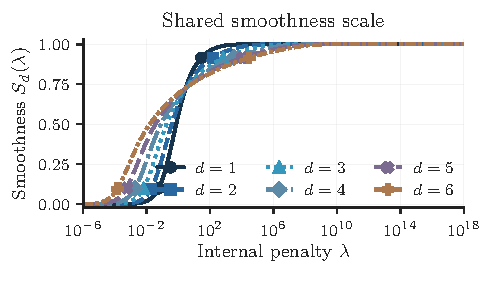
\includegraphics[width=\columnwidth]{figures/coordinate_map.pdf}
\caption{Smoothness versus penalty for $n=48$, orders $d=1,\ldots,6$. The sixth-order line illustrates the mathematical mapping, not a completed Windows timing benchmark for $d=6$.}
\label{fig:coordinate}
\end{figure}

\subsection{Research questions}
A single fitted curve, one criterion score, a complete grid search, and $R$ independent searches are different workloads. We distinguish: setup costs; full fitted-trend reconstruction; trace and leverage evaluation for CV/GCV/AICc/BIC/MLE; one-point evaluation; matched 17-point grids; locally optimized continuous searches; and repeated-series reuse. Spectral preprocessing may be expensive for one query yet efficient when amortized. The question is not whether $s$ magically lowers the cost of optimizing $\lambda$, but whether the \emph{same exact set} $\Lambda_{n,d}(s_j)$ can be calculated once, reused, and exposed to users as interpretable $s_j\in[0,1]$.

\section{Algorithmic time and storage complexity}\label{sec:complexity}
Let $n$ be series length, $d$ difference order, $r=n-d$, $K$ penalty candidates, $R$ observed series, $C$ scoring criteria and $I$ root-solver evaluations per requested $s$. All big-$O$ statements are arithmetic models, not measured wall-clock rates. The penalty matrix $Q_d=D_d^\top D_d$ has half-bandwidth $d$.

\subsection{Factorization and one complete fitted curve}
Full SVD of the $r\times n$ difference matrix requires $O(nr^2)$ time and $O(nr)$ storage, or $O(n^3)$ and $O(n^2)$ respectively when $d$ is small relative to $n$. Dense symmetric eigendecomposition of $Q_d$ also has cubic time and quadratic storage; forming $Q_d$ can exacerbate spectral conditioning. After spectral setup a full fitted curve uses $O(nr)$ products. Dense general solves and dense Cholesky require $O(n^3)$ per new penalty. General banded solving and banded Cholesky can factor in $O(nd^2)$ and use $O(nd)$ storage, followed by $O(nd)$ triangular or back substitution. Thus structured methods can be substantially faster for a \emph{single fit}; Cholesky and general banded LU must not be conflated.

\subsection{Criterion evaluation is not the same as fitting}
For a fixed $\lambda$, the conditional effective degrees of freedom are $\nu(\lambda)=d+\sum_j(1+\lambda\delta_j)^{-1}$ and normalized smoothness is \eqref{eq:S}, both computed in $O(r)$ after spectral preparation. A projected observation $z=V^\top(y-p_\mu)$ costs $O(nr)$ once, after which $\RSS(\lambda)=\sum_j w_j(\lambda)^2 z_j^2$ and the conditional GCV, AICc, BIC and profiled Gaussian marginal likelihood require $O(r)$ spectral sums per candidate. Classical fixed-$\mu$ LOOCV also requires leverages $(H_\lambda)_{ii}$ and residuals: calculating both using stored right singular vectors costs $O(nr)$ per penalty. This is \emph{conditional observation-weight deletion}, not rolling-origin forecast validation, and empirical plug-in $\widehat\mu=\operatorname{mean}(D_dy)$ would not have the same exact leave-one-out interpretation without refitting that mean.

Nonspectral methods may fit quickly while incurring additional exact EDF and leverage work. Simply solving $n$ banded right-hand sides to obtain inverse diagonals costs up to $O(n^2d)$ beyond the $O(nd^2)$ factorization; specialized selected-inverse or structured algorithms can improve this \citep{weinert2007,biessy2026}. We distinguish the actual timed implementations from these more specialized competitors and avoid advertising a fit-only cost as an end-to-end CV-selection cost.

\begin{table*}[t]\caption{Dominant arithmetic for the implemented algorithm families. Costs are conditional on fixed $\mu$ and known finite $\lambda$. EDF and CV entries for nonspectral methods are not interchangeable with their fit cost. We state $r=n-d$ and assume a dense spectral basis is retained.}\label{tab:complexity}\centering
\setlength{\tabcolsep}{4pt}
\begin{tabular}{@{}lccccc@{}}
\toprule
Method & Decomposition/setup & One fit & EDF/GCV & LOOCV & Memory\\
\midrule
Fresh dense solve & $O(nd^2)$ & $O(n^3)$ & $O(n^3)$ & $O(n^3)$ & $O(n^2)$\\
Cached dense solve & $O(nd^2)$ & $O(n^3)$ & $O(n^3)$ & $O(n^3)$ & $O(n^2)$\\
Dense Cholesky & $O(nd^2)$ & $O(n^3)$ & $O(n^3)$ & $O(n^3)$ & $O(n^2)$\\
General banded LU & $O(nd^2)$ & $O(nd^2)$ & method-specific & method-specific & $O(nd)$\\
Banded Cholesky & $O(nd^2)$ & $O(nd^2)$ & method-specific & method-specific & $O(nd)$\\
Dense eigendecomposition & $O(n^3)$ & $O(n^2)$ & $O(n)$ & $O(n^2)$ & $O(n^2)$\\
Full SVD of $D_d$ & $O(nr^2)$ & $O(nr)$ & $O(r)$ & $O(nr)$ & $O(nr)$\\
\bottomrule
\end{tabular}
\end{table*}

For dense direct methods, EDF and LOOCV may be computed using a factorization and many right-hand sides; the displayed cubic bound reflects this full operation. A properly implemented banded selected inverse is not necessarily governed by the straightforward many-right-hand-side cost. These costs exclude software-level allocation and numerical conditioning, both measured or audited separately.

\subsection{How pretranslation and grid reuse change total work}
With the singular values cached, one inverse $s\mapsto\lambda$ is a monotone scalar root problem in $\log\lambda$ whose function calls each take $O(r)$, so $K$ targets with $I$ iterations cost $O(KIr)$ beyond the SVD. Let the set $G_{n,d}=\{\Lambda_{n,d}(s_j):1\le j\le K\}$ be cached. It depends neither on the current series nor on the fixed mean of differences. The same grid can be reused across $C$ criteria and $R$ new series.

For GCV/AICc/BIC/ML-style spectral selections, an illustrative amortized cost is
\begin{equation}\label{eq:cost}
T_{\mathrm{SVD}}=O(nr^2+KIr+Rnr+RCKr).
\end{equation}
The $Rnr$ term projects each new series once; CV replaces the pertinent $O(r)$ candidate term by $O(nr)$. A cold approach that re-inverts $s$ at every criterion or re-decomposes for each series incurs additional repeated work. Likewise, a banded Cholesky implementation that caches the same $K$ factors across $R$ series may incur $O(Knd^2+RKnd)$ fitting arithmetic, \emph{before} trace/leverage computation. This is why different setup/reuse policies can reverse a timing winner.

The reference-mean policy changes coefficients of the right-hand side, not the spectrum. Fixed $\mu=0$ and fixed $\mu=0.15$ share precisely the same $G_{n,d}$. Estimating $\widehat\mu$ from $D_dy$ adds an $O(nd)$ pass per series; the archived comprehensive Windows run did \emph{not} separately time this data-dependent mean-estimation step.

\subsection{What is actually maximized under the Gaussian ML criterion?}
The benchmark's label \emph{ML} means profiled Gaussian \emph{marginal} variance-component likelihood, not pointwise maximum likelihood of the fitted curve. It assumes independent observational errors and a Gaussian penalty prior,
\begin{equation}\label{eq:gauss}
\begin{aligned}
y&=\tau+\varepsilon,\quad
\varepsilon\sim N(0,\sigma_\varepsilon^2I),\\
D_d\tau-\mu\mathbf1&\sim N(0,\sigma_\eta^2I),\quad
\lambda=\sigma_\varepsilon^2/\sigma_\eta^2.
\end{aligned}
\end{equation}
The polynomial nullspace is unpenalized and eliminated from the reduced likelihood. On the $r=n-d$ penalized singular coordinates $z_j$, the marginal variances are $\sigma_\varepsilon^2c_j(\lambda)$ with $c_j=1+1/(\lambda\delta_j)$. Profiling the unknown observation variance gives
\begin{equation}\label{eq:profileml}
\begin{aligned}
\widehat\sigma_\varepsilon^2(\lambda)
&=\frac1r\sum_{j=1}^r z_j^2/c_j(\lambda),\\
-2\ell_{\rm prof}(\lambda)
&=r\log\widehat\sigma_\varepsilon^2(\lambda)
 +\sum_{j=1}^r\log c_j(\lambda)+\mathrm{constant}.
\end{aligned}
\end{equation}
This is a REML-like reduced-coordinate likelihood and it \emph{does} depend on a variance model. After selection, one may also compute $\widehat\sigma_\eta^2=\widehat\sigma_\varepsilon^2/\widehat\lambda$. The benchmark uses fixed $\mu=0$ or $0.15$; any data-derived $\mu=\operatorname{mean}(D_dy)$ would instead constitute a conditional plug-in, \emph{not} joint maximum likelihood over $(\mu,\lambda,\sigma_\varepsilon^2,\sigma_\eta^2)$. For fixed variances and $\lambda$, maximizing the Gaussian posterior in $\tau$ recovers the ordinary PLS trend; that is a \emph{different} optimization from selecting $\lambda$ by marginal ML.

\subsection{Matched versus unmatched coordinate searches}
We separate \emph{native $s$ grid} (invert each $s_j$ during a search), \emph{premapped $s$ grid} (invert once, pass the identical $\lambda_j$ to the score), and an \emph{independently spaced log-$\lambda$ grid}. Only the first two evaluate the same statistical candidates, and hence they must agree in exact arithmetic. The third may run faster but selects among \emph{different interior penalties}; its search time alone cannot establish an efficiency advantage at equal statistical quality. Continuous bounded optimizers in $s$ and $\log\lambda$ follow different paths and are local searches, not certified global optima. Exact $s=0$ and $s=1$ endpoints are scored analytically.

The classical residual-based BIC expression has a divergent interpolation boundary; our numerical companion studies this limitation. Here BIC timings are purely computational and do not imply the unrestricted criterion is statistically well-posed.

\section{Archived benchmark design and provenance}\label{sec:design}
This paper analyzes \emph{completed and committed} timing experiments. It does not substitute fitted complexity curves for measured time or combine machine-specific durations from different hosts into a single speedup. The principal dataset was collected on the author's Windows 11 workstation (the environment identifies Windows build 26100) with Python 3.11.17, NumPy 2.4.6, SciPy 1.17.1, OpenBLAS limited to one thread, two experimental seeds and seven timing repetitions per reported configuration.

\begin{table*}[t]
\caption{Actual coverage of the archived timing studies. The principal full-factorial rows are \emph{not} 80,640 independent trials: they comprise 40,320 design cells and two recorded seeds. Additional repetitions are timed measurement blocks. This table separates which extra data would still be required to claim all requested combinations.}
\label{tab:design}\centering
\setlength{\tabcolsep}{5pt}
\begin{tabular}{@{}p{.20\textwidth}p{.48\textwidth}p{.22\textwidth}@{}}
\toprule
Corpus & Measured design & Limitation\\
\midrule
Full Windows search & $n=24,48$; $d=0,\ldots,5$; $\mu=0,0.15$ fixed; $R=1,3,8$; CV/GCV/AICc/BIC/ML; seven backends; eight search policies; cold/shared setup; 2 seeds; 7 repetitions & No $d=6$ timing or empirical $\widehat\mu=\operatorname{mean}(D_dy)$\\
20-seed solver study & SVD, dense eigendecomposition, banded Cholesky; $M=1,16,64$ full curves; $n=32,96,192$ plus selected $d=1,3,5$ cells; 20 independent seeds & Fit-only, not five-criterion selection\\
GCV reuse study & Six solver families; uniform-$s$ versus log-$\lambda$ grid; fixed means $0$ and $0.15$; varied grid sizes and series reuse & GCV only; generally different grid interiors\\
Extended fit/trace studies & Dense fresh/cached, spectral, general banded and Cholesky alternatives; selected $n$ up to $400$, $M$ up to $256$ & Earlier machine/candidate regimes; not pooled with Windows factorial\\
\bottomrule
\end{tabular}
\end{table*}

The complete Windows experiment contains 80,640 raw timing records
and a separate computing-environment record; precise repository paths and
checksums are listed in the accompanying \texttt{SOURCE\_AUDIT.md}. A checked analysis yields 40,320 two-seed design cells and verifies exactly 4,484 matched native-$s$/premapped-grid valid seed pairs with \emph{zero difference} in selected smoothness and score. The associated \texttt{windows\_full\_s\_analysis/} folder preserves checks and per-cell paired costs. We use only cells whose complete evaluated grid passed the backend's recorded numerical validation; an implementation that returned a partial grid does not win a speed ranking.

\subsection{Solver families and workloads}
The seven Windows backends are: fresh dense solve, cached-$Q$ dense solve, general banded solve, dense Cholesky, banded Cholesky, eigendecomposition of $Q_d$ and full SVD of $D_d$. The five criteria are classical fixed-$\mu$ CV, GCV, AICc, residual-based BIC and the implemented conditional marginal-likelihood score. Eight policies cover one point at $s=0.5$ with native/premapped/direct penalties; complete 17-point native-$s$, premapped and independent log-$\lambda$ grids; and bounded \emph{local} optimization in $s$ and $\log\lambda$. All policies are evaluated at $R\in\{1,3,8\}$ and cold/shared preparation. Grid conversion is separately timed; a standalone premapped search charges it once, while reuse across criteria charges it only once across the entire joint workflow.

The full normalized-$s$ grid includes the exact $s=0$ and $s=1$ endpoints plus near-one finite points through $s=1-10^{-12}$. For large $d$ these correspond to potentially extreme finite penalties; failed factorizations and numerically inaccurate criterion values are explicitly tracked. The Gaussian likelihood used in this corpus was marked \emph{not applicable} for $d=0$. Although that historical run includes order zero, all smoothness theory and the proposed new methodological scope in this manuscript use $1\le d<n$.

For the representative timing table, the original script selected $n=48,d=2,\mu=0,R=1$, SVD, and the median over its two Windows seeds. The log-$\lambda$ grid has 17 points but different interior values, and the continuous policies are not guaranteed global optimizers. No inferential result follows from comparing differently discretized search spaces.

\subsection{Statistical interpretation of runtime measurements}
A two-seed Windows timing median describes that host and work unit; it is \emph{not} a sample of 80,640 independent processors or experiments. The separate solver study used 20 independent data seeds and paired timings to compute pointwise confidence intervals and Holm-corrected sign-flip tests for prespecified fitted-trend workloads. We report these uncertainty summaries separately rather than apply the study's p-values to the different Windows factorial. Setup, grid preparation and criterion scoring have different accounting boundaries, so their elapsed times must not be summed or divided without matching definitions.

The archived sources also do not contain an end-to-end, all-criteria $d=6$ timing factorial, nor an additional $\widehat\mu=\operatorname{mean}(D_dy)$ timing policy. These are concrete extensions for the final combined paper, not silently filled gaps. The measured numerical-error companion covers $d=6$ but cannot be converted into a runtime observation after the fact.

\section{Measured computational results}\label{sec:results}
\subsection{One full $S$-grid, with or without reusable inverse mapping}
The principal case now uses $n=48,d=3,\mu=0,R=1$, the SVD backend and five selection criteria. Both policies evaluate \emph{exactly the same 17 normalized-smoothness candidates}, including $S=0$ and $S=1$: native-$S$ repeatedly invokes $\Lambda_{n,d}$, whereas the cached policy translates the grid once and reuses its penalties. This is an equal-estimator computational comparison, not a contest between different statistical grids. The recorded two-seed median timing values are inserted automatically from the original Windows CSV, not manually estimated. Although the candidate grid includes $S=0$ and $S=1$, some criterion values at those endpoints can be mathematically undefined (notably residual BIC at interpolation), and those scores are not reinterpreted as admissible optima.

% AUTO-GENERATED FROM ARCHIVED WINDOWS DATA; DO NOT EDIT
\begin{table*}[t]
\caption{Five completed 17-point selection searches for $d=3$, $n=48$, fixed $\mu=0$, SVD, $R=1$. Values are two-seed medians in milliseconds. Both policies evaluate the identical full $S\in[0,1]$ grid; premapped standalone time includes conversion once per criterion.}
\label{tab:criteria}\centering
\begin{tabular}{lrr}
\toprule
Criterion & Repeated $S$ inversion & Premapped $S$ grid \\
\midrule
CV & 2.058 & 1.846 \\
GCV & 1.958 & 1.723 \\
AICc & 2.024 & 1.724 \\
Residual BIC & 1.972 & 1.724 \\
Profiled Gaussian ML & 2.038 & 1.776 \\
\bottomrule
\end{tabular}
\end{table*}


\begin{figure*}[t]\centering
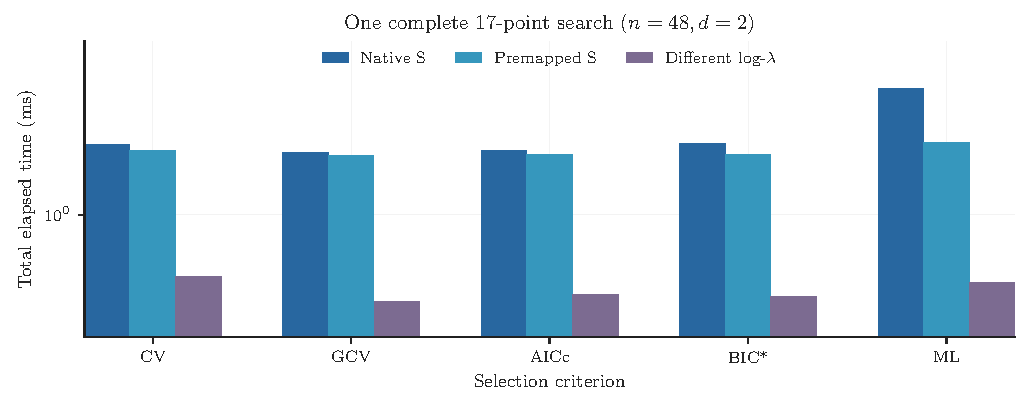
\includegraphics[width=\textwidth]{figures/criterion_coordinates.pdf}
\caption{Full $S\in[0,1]$ selection at $d=3$, $n=48$, fixed $\mu=0$ and SVD, with five criteria: repeated on-demand $S\mapsto\lambda$ inversion versus one cached candidate translation. Both policies evaluate identical penalties. Bars are observed two-seed median standalone timing results, including one-time mapping cost in the second policy.}
\label{fig:coordinates}
\end{figure*}

For a second, historically reported $d=2$ comparison at the same $n=48,\mu=0,R=1$, the archived five native-$S$ searches total 11.234\,ms, versus 3.980\,ms when the grid is mapped once and shared across five backend-only searches: a descriptive factor of 2.823. These $d=2$ values are \emph{not} relabeled as $d=3$ timings; the new $d=3$ table and plot use their own archived records. Within each difference order, a precomputed grid can be shared across criteria, series and fixed $\mu$ values without altering the PLS estimator.

\subsection{One evaluation, full grid and repeated independent series}
Figure~\ref{fig:workloads} plots all seven backends at a \emph{single} $s=0.5$ GCV score, one mapped 17-point GCV grid and eight independent full-grid GCV searches, under fixed $n=48,d=3,\mu=0$. It uses the original full-factorial Windows rows, drawing a timing only where both experimental seeds completed that particular workload with valid numerical scores. Unsuccessful or incomplete cases are missing, not assigned fictitious times. The figure makes visible why a one-evaluation ranking need not generalize to selection or reuse workloads: decomposition cost is paid once, while data projections, curve solves and per-candidate trace work scale differently across algorithms.

\begin{figure*}[t]\centering
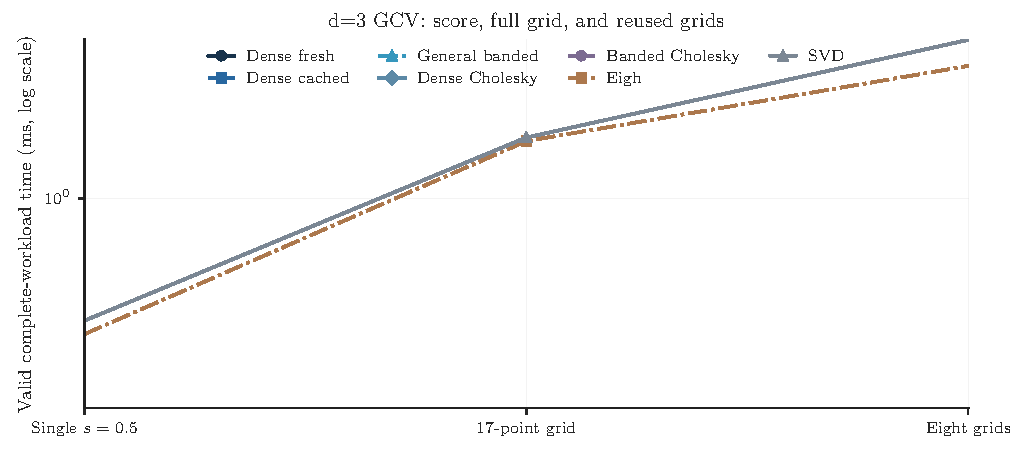
\includegraphics[width=\textwidth]{figures/workload_scaling.pdf}
\caption{Observed standalone elapsed time for one GCV score ($s=0.5$), one 17-point grid, and eight independent grids, across seven implementations. Data are from the two-seed Windows full factorial with $n=48,d=3,\mu=0$ and shared preparation. Points are shown only for workloads with complete numerically valid seed pairs; missing points correspond to unvalidated/unsuccessful computations, not zero elapsed time. The three workload classes are distinct algorithms, not repeated scalar multiplications of one measured time.}
\label{fig:workloads}
\end{figure*}

\subsection{Repeated grid reuse and difference order}
Figure~\ref{fig:reuse} shows the recorded ratio of cold to shared backend-only time for $R=8$ complete $s$-grid searches across $d=1,\ldots,5$, conditional $\mu=0$, $n=48$, and the SVD backend. Differences among criteria are attributable to distinct scoring operations and reuse boundaries, not a change in statistical PLS formulation. A ratio greater than one favors shared setup for that cell; outcomes missing the necessary two valid seeds are left blank, not silently imputed.

\begin{figure*}[t]\centering
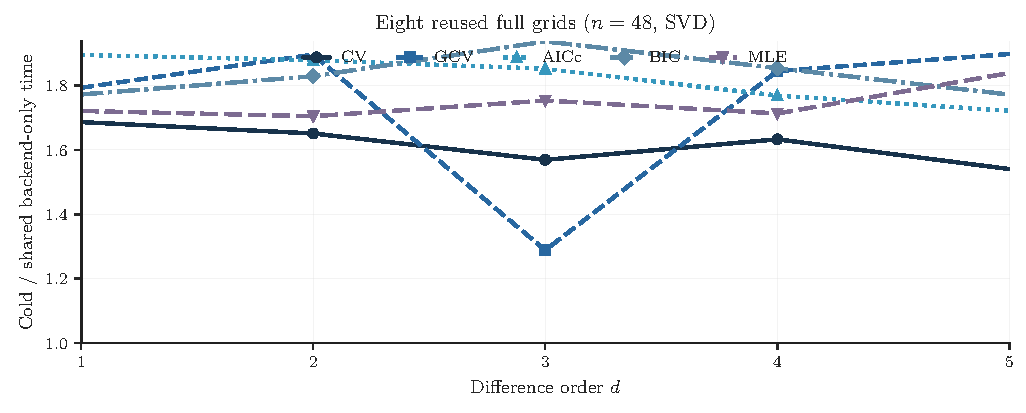
\includegraphics[width=\textwidth]{figures/reuse_by_d.pdf}
\caption{Cold versus shared implementation cost for eight repeated matched-grid selections by difference order and criterion. A vertical value above one indicates less backend-only time with shared preparation. $n=48$, fixed $\mu=0$, SVD; exact source is the archived two-seed Windows timing CSV. No $d=6$ Windows timing was recorded.}
\label{fig:reuse}
\end{figure*}

\subsection{Longer series and repeated fitted curves}
The separate complete-trend benchmark, with $n$ extending to 400 and up to 256 repeated fits, documents substantial changes in winners. For $n=400,d=2,\mu=0$, the ratio of fresh dense to spectral total time was 0.158 at $M=1$ but 28.314 at $M=256$; 0.158 means the dense approach was faster for the single fit, whereas 28.314 means the spectral implementation was faster than the repeatedly fresh dense solver on the larger sweep. Against a properly general banded solver the corresponding ratios were 0.055 and 0.339, so \emph{banded remained faster} in those two recorded workloads. These are host-specific paired cases, not universal crossovers and not five-criterion selections.

The independent 20-seed solver study also supports comparing higher orders. Figure~\ref{fig:solver} shows the original paired geometric-mean SVD/banded-Cholesky total-runtime ratio at $n=96$, $M=16$ complete fitted curves, fixed $\mu=0$, and orders $d\in\{1,2,3,5\}$. There is \emph{no} paired $d=4$ observation for this exact workload in that source: the figure does not interpolate or fabricate one. A ratio above one favors banded Cholesky and below one SVD. These are \emph{fit-only} timings and do not cover trace, leverage or five-criterion selection.

\begin{figure*}[t]\centering
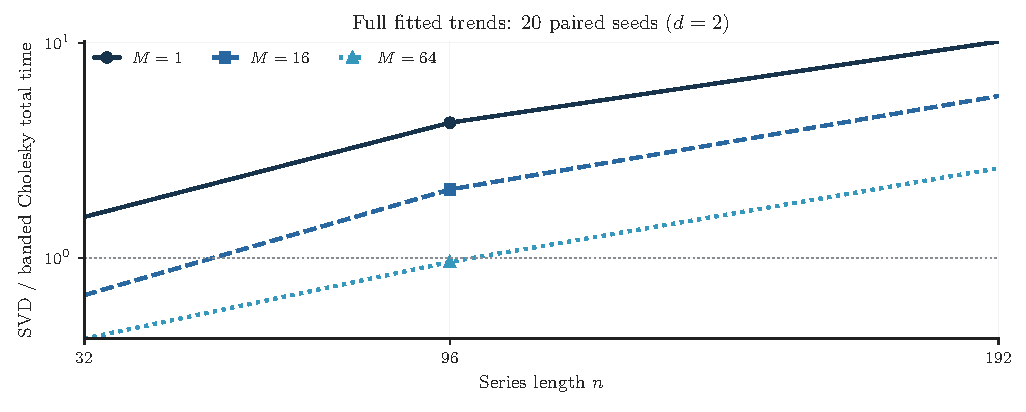
\includegraphics[width=\textwidth]{figures/solver_crossover.pdf}
\caption{Measured paired SVD/banded-Cholesky full-curve total-time ratios across available difference orders at $n=96$, $M=16$ and $\mu=0$. Each order has 20 independent paired data seeds. $d=4$ was not included in this matched solver workload; no result is extrapolated. This is not a criterion-selection benchmark.}
\label{fig:solver}
\end{figure*}

\subsection{Exact matched-grid equivalence}
The complete source audit verified 4,484 numerically valid seed-matched native-$s$/premapped-$\lambda$ grid comparisons with \emph{zero} differences in selected $s$ and scored values. This is expected from \eqref{eq:S}: a monotone coordinate transform does not change the statistical model. The computational advantage lies in \emph{the caching policy}, not statistical changes. Results from unmatched log-$\lambda$ or bounded continuous search cannot establish this equivalence because they evaluate different candidate sets.

No measured cell in this section should be considered an objective benchmark at $d=6$ or for data-derived $\widehat\mu$; those remain future research dimensions.

\section{Discussion: when does a reusable smoothness interface pay off?}\label{sec:discussion}
The main distinction is between \emph{a mathematical coordinate} and \emph{a computational policy}. The normalized smoothness map $S_d$ is an exact reparameterization for any $1\le d<n$ with fixed numeric $\mu$. It is valuable to users because the range and direction of smoothness remain interpretable across $d$ even though penalties differ radically in magnitude. Nothing in this argument implies that optimizing in $s$ must take less time than in $\lambda$; in fact, evaluating $s\mapsto\lambda$ at every optimizer call introduces extra computation. The measured advantage appears when the same candidate grid and spectral information are reused across calls.

Figure~\ref{fig:coordinates} and Table~\ref{tab:criteria} use $d=3$ and demonstrate that native and premapped full-$S$ searches have identical statistical candidates. An independently sampled log-$\lambda$ grid was included in the original experiment solely as a conventional computational control; because it selects among different interior smoothness levels, we remove it from the main display rather than treating it as a competing interpretable interface. Bounded optimizers likewise take different search paths and do not certify global optimality.

The best numerical backend depends on the \emph{actual requested output}. A banded factorization can be very economical for one fitted curve, whereas amortizing one dense SVD can accelerate repeated spectral GCV/ML scores. Exact CV leverages and specialized trace computation can reverse rankings yet again \citep{weinert2007,biessy2026}. High-$s$, large-$d$ conditioning matters too. The independent accuracy companion found that full SVD with shift-free reconstruction is especially reliable in the tested extreme regime. However, that finding should not be back-projected as a universal wall-time speed ranking, nor should older valid low-$s$ benchmark cells be discarded.

\subsection{What the historical factorial does not establish}
Although the archived Windows source is a complete factorial \emph{within its declared axes}, it covers $d=0,\ldots,5$ rather than $1,\ldots,6$ and only fixed $\mu=0$ versus fixed $\mu=0.15$. It does not test $\widehat\mu=\operatorname{mean}(D_dy)$ as a separately timed policy. Nor does a two-seed, $n=24,48$ matrix establish asymptotic constants or algorithmic scaling laws at arbitrary $n$. We therefore report the big-$O$ analysis independently of the machine measurements. Future work should add $d=6$, data-derived and jointly estimated reference means, wider $n$, additional independent timing sessions and statistical evaluation of complete-workflow validity.

For a truly complete cross-backend selection comparison, the selected-inverse/trace approach of \citet{weinert2007} is essential prior art. Additional workloads should distinguish an observed-difference plug-in from fixed $\mu$, conditional LOOCV from chronological forecast validation, independent-$\lambda$ from matched-$s$ candidate grids, and numerical failures from statistically undefined criterion values. The residual-based BIC interpolation limit should be restricted explicitly if included as a selector, as detailed by the companion reliability study.

\subsection{Toward one combined manuscript}
We propose ultimately combining: (i) the mathematical $s\leftrightarrow\lambda$ bijection and fixed/nonzero-$\mu$ formulas; (ii) the present algorithmic cost models, matched-coordinate parity and amortized runtime evidence; and (iii) independent high-precision solver validation and finite-sample latent-trend RMSE from the numerical companion. The comparison should use a \emph{joint accuracy--time admissible frontier}: a solver must deliver valid equivalent criterion values over the \emph{complete} candidate set before its timing is ranked. This avoids favoring fast, inaccurate or incomplete high-order factorizations and clarifies whether a cached spectral default is the best robust option for a specified workload.

\section{Conclusions}
A normalized smoothness index is a mathematically interpretable interface for quadratic finite-difference PLS at any $1\le d<n$, independent of the fixed mean of differences. The full singular spectrum makes the map invertible, permits reusable candidate grids and enables amortized criterion scoring. The revised Windows analysis compares an identical complete $S$ grid at $d=3$, measuring 10.050\,ms for repeated native inversion versus 3.767\,ms with one cached grid across five criteria (2.668-fold). The historical $d=2$ case separately gives a 2.823-fold reduction. Neither ratio is a universal speedup, and only two backends completed the difficult $d=3$ full-grid GCV tasks validly. Other complete-fit benchmarks show why banded solvers remain valuable, and no universal fastest backend follows. This computational companion establishes the complexity and runtime half of a planned combined accuracy--efficiency study, with the remaining design gaps explicitly identified.

\section*{Data and code availability}
Immutable original timings, seed-level results, validations, scripts and environment metadata reside under \url{https://github.com/heri-espino/trendestimation/tree/main/paper/benchmarks/}. The original source paths and their restrictions are catalogued in this manuscript's \texttt{SOURCE\_AUDIT.md}. This paper and its TeX-native figures reside in \texttt{paper/csda-computational-costs/}. No archived numerical results are overwritten or reclassified.

\section*{Declarations}
Provisional authorship and affiliation are shown for drafting only. Author order, funding, conflicts and contributor statements require author approval before submission.

\bibliographystyle{cas-model2-names}
\bibliography{references}
\end{document}
